% !TEX root = ../presentation.tex

\subsection[Matrix Fisher]{Attitude Uncertainty using Matrix Fisher}


\begin{frame}
\frametitle{Matrix Fisher Distribution on $\SO$}
\begin{itemize}
\item Matrix Fisher Distribution: $\mathcal{M}(F)$
	\begin{itemize}
	\item Probability density defined by a \Emph{matrix parameter} $F\in\Re^{3\times 3}$
\only<1>{

	    \centerline{
	    \begin{beamercolorbox}[wd=10cm,sep=0.0cm,center,rounded=true,shadow=true]{numerical}
		$\displaystyle R\sim\mathcal{M}(F)\quad\Leftrightarrow\quad p(R) \propto  \exp(\mathrm{tr}[F^T R])$
		\end{beamercolorbox}}
		}
\only<2->{

	    \centerline{
	    \begin{beamercolorbox}[wd=10cm,sep=0.0cm,center,rounded=true,shadow=true]{numerical}
                {\small$\displaystyle p(R) = \frac{1}{c(F)}  \exp(\mathrm{tr}[F^T R])$}
		\end{beamercolorbox}}
}
\pause
	\item Normalizing constant $c(F)$ introduced for $\int_{\SO} p(R) dR =1$
%	\item Haar measure $dR$ scaled such that $\int_{\SO} dR =1$
	\item Comparable to a \Emph{Gaussian distribution on $\Re^3$} defined by 9 parameters
	\end{itemize}
\pause
\only<1-3>{\item Singular Value Decomposition of $F$

	\centerline{
	\begin{beamercolorbox}[wd=\textwidth,sep=0.0cm,center,rounded=true,shadow=true]{numerical}
	\vspace*{-0.5cm}
	\begin{align*}
	F & = U' S' (V')^T\\
	&= \begin{bmatrix} & & \\ u'_1 & u'_2 & u'_3 \\ & & \end{bmatrix}
	\begin{bmatrix} s'_1 & 0 & 0\\ 0 & s'_2 & 0 \\ 0 & 0 & s'_3 \end{bmatrix}
	\begin{bmatrix} & (v_1')^T & \\ & (v_2')^T & \\ & (v_3')^T & \end{bmatrix}
	\end{align*}\vspace*{-0.3cm}
	\end{beamercolorbox}}

	\begin{itemize}
	\item Positive singular values: $s_1'\geq s_2'\geq s_3'\geq 0$
	\item $U',V'\in\Re^{3\times 3}$ are orthogonal, but not neccessarily in $\SO$ . 
	\end{itemize}}
\only<4>{\item \Emph{\textit{Proper}} Singular Value Decomposition of $F$

	\centerline{
	\begin{beamercolorbox}[wd=\textwidth,sep=0.0cm,center,rounded=true,shadow=true]{numerical}
	\vspace*{-0.5cm}
	\begin{align*}
	F & = U S V^T\\
	&= \begin{bmatrix} & & \\ u'_1 & u'_2 & \Emph{\mathrm{det}[U']}u'_3 \\ & & \end{bmatrix}
	\begin{bmatrix} s'_1 & 0 & 0\\ 0 & s'_2 & 0 \\ 0 & 0 & \Emph{\mathrm{det}[U'V']}s'_3 \end{bmatrix}
	\begin{bmatrix} & (v_1')^T & \\ & (v_2')^T & \\ & \Emph{\mathrm{det}[V']}(v_3')^T & \end{bmatrix}
	\end{align*}\vspace*{-0.3cm}
	\end{beamercolorbox}}
	
	\begin{itemize}
	\item $s_1\geq s_2\geq |s_3|\geq 0$,\quad $s_1+s_2\geq s_1+s_3\geq s_2+s_3\geq 0$
	\item $U,V\in\SO$
	\end{itemize}}
		
\end{itemize}
\end{frame}
<`0`>
\begin{frame}
\frametitle{Matrix Fisher Distribution on $\SO$}
\begin{itemize}
\item Shape of Matrix Fisher Distribution with $F=USV^T$
	\begin{itemize}
	\item \Emph{Mean attitude} : $UV^T$
	\item \Emph{Principal axes} : columns of $U$
	\item \Emph{Dispersion} along the $i$-th principal axis: $s_j+s_k$
	\end{itemize}
\vspace*{0.3cm}\pause
\end{itemize}
\vspace*{-0.3cm}
\begin{columns}[t]
\begin{column}{0.32\textwidth}
\only<1>{
\begin{tikzpicture}
\node[opacity=0.3,outer sep=0pt,inner sep=0pt] at (0,0) {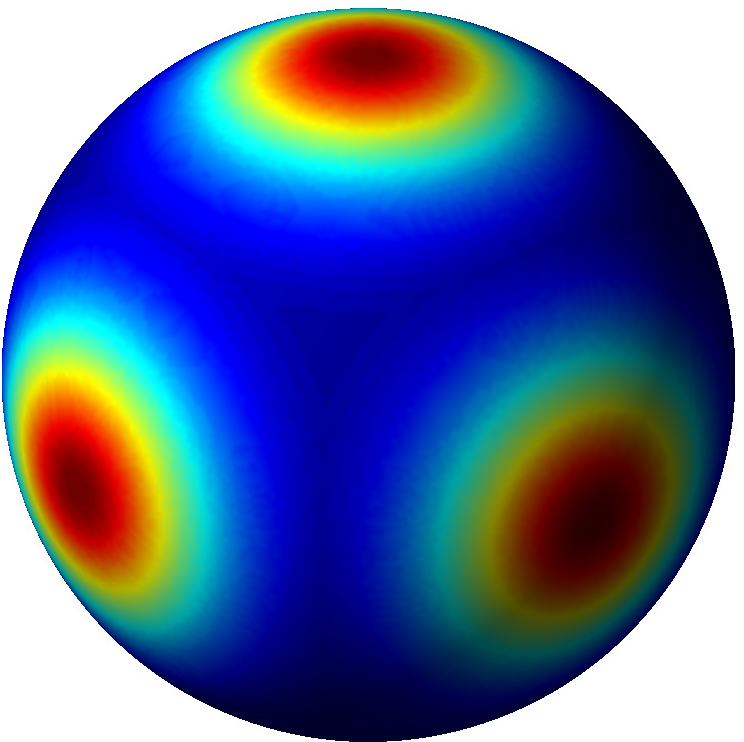
\includegraphics[height=0.4\textheight,width=1\columnwidth, keepaspectratio]{figures/2017AAS_matrix_fisher/TAC16_vis_1}};
\end{tikzpicture}
\centerline{\footnotesize $F_1=5I_{3\times 3}$}
\centerline{\footnotesize $U_1V_1^T=I_{3\times 3},\, U_1=I_{3\times 3}$}
\centerline{\footnotesize $S_1=\mathrm{diag}[5,5,5]$}
}
\only<2->{
\begin{tikzpicture}
\node[opacity=1,outer sep=0pt,inner sep=0pt] at (0,0) {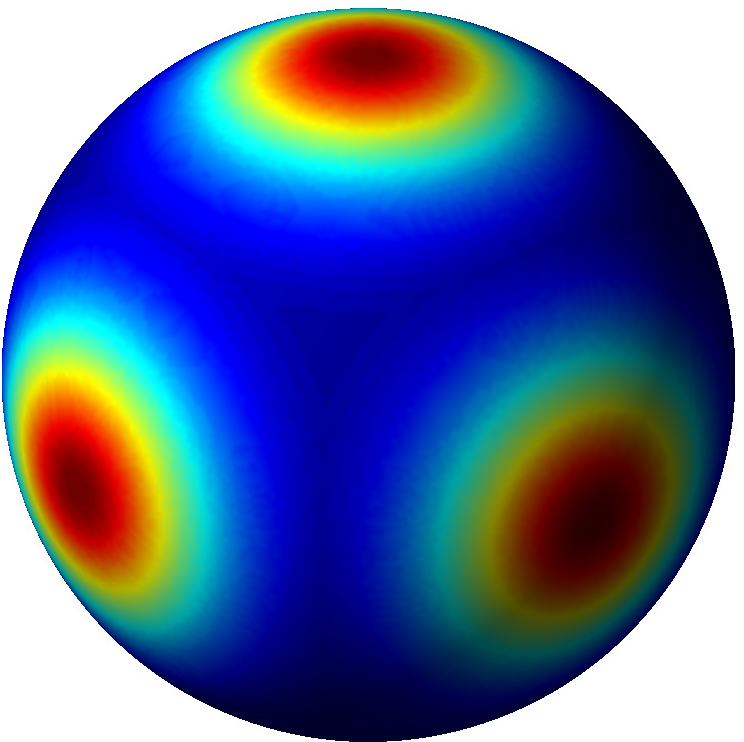
\includegraphics[width=1\columnwidth,height=0.4\textheight, keepaspectratio]{figures/2017AAS_matrix_fisher/TAC16_vis_1}};
\end{tikzpicture}
\centerline{\footnotesize $F_1=5I_{3\times 3}$}
\centerline{\footnotesize $U_1V_1^T=I_{3\times 3},\, U_1=I_{3\times 3}$}
\centerline{\footnotesize $S_1=\mathrm{diag}[5,5,5]$}
}
\end{column}
\pause
\begin{column}{0.32\textwidth}
\only<1,2>{
\begin{tikzpicture}
\node[opacity=0.3,outer sep=0pt,inner sep=0pt] at (0,0) {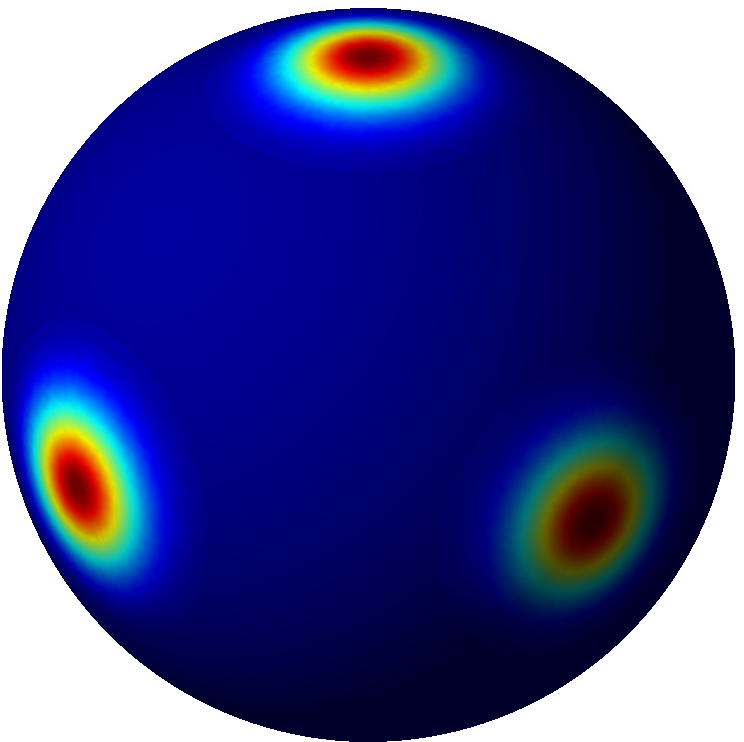
\includegraphics[width=1\columnwidth,height=0.4\textheight,keepaspectratio]{figures/2017AAS_matrix_fisher/TAC16_vis_2}};
\end{tikzpicture}
}
\only<3->{
\begin{tikzpicture}
\node[opacity=1,outer sep=0pt,inner sep=0pt] at (0,0) {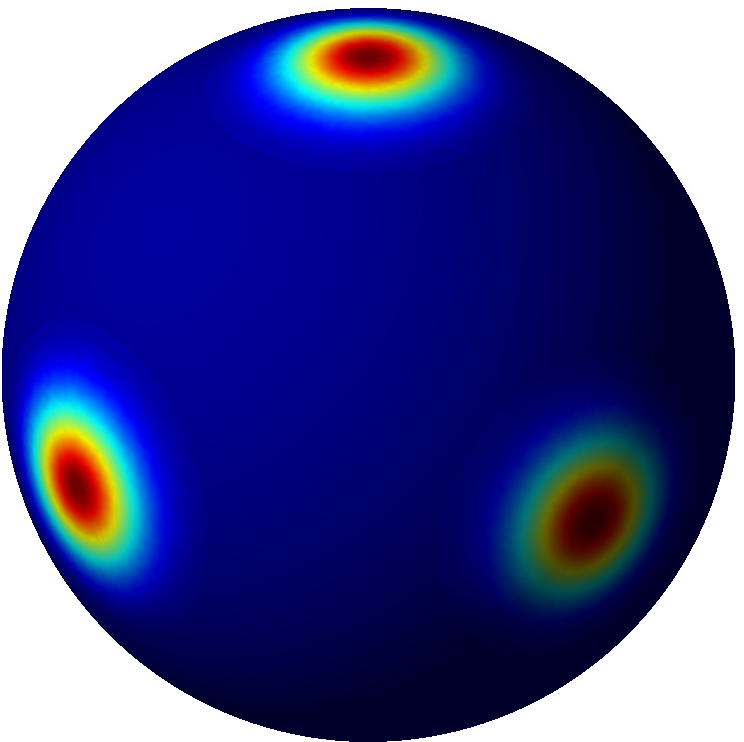
\includegraphics[width=1\columnwidth,height=0.4\textheight,keepaspectratio]{figures/2017AAS_matrix_fisher/TAC16_vis_2}};
\end{tikzpicture}
}
\centerline{\footnotesize $F_2=20I_{3\times 3}$}
\centerline{\footnotesize $U_2V_2^T=I_{3\times 3},\, U_2=I_{3\times 3}$}
\centerline{\footnotesize $S_2=\mathrm{diag}[20,20,20]$}
\end{column}
\pause
\begin{column}{0.32\textwidth}
\only<1,2,3>{
\begin{tikzpicture}
\node[opacity=0.3,outer sep=0pt,inner sep=0pt] at (0,0) {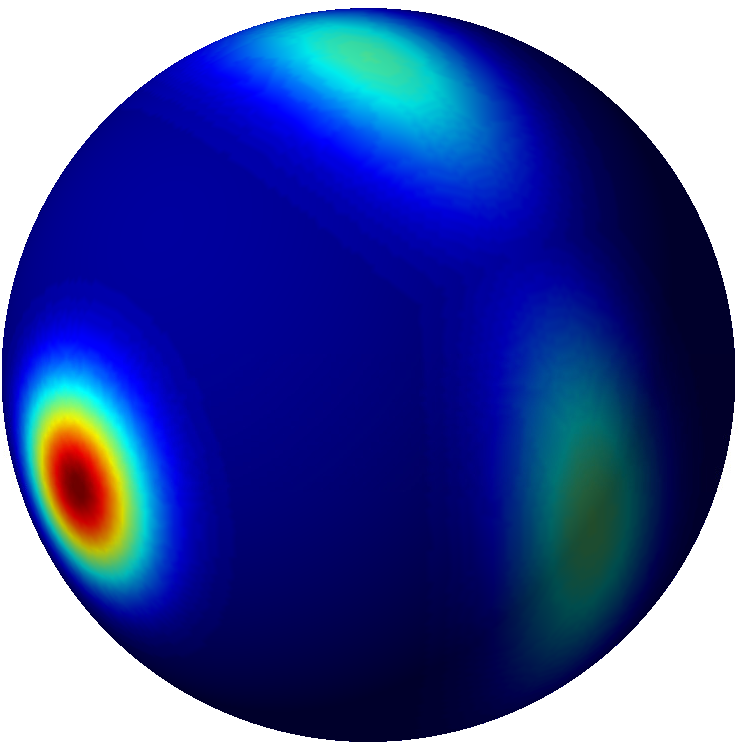
\includegraphics[width=1\columnwidth,height=0.4\textheight,keepaspectratio]{figures/2017AAS_matrix_fisher/TAC16_vis_3}};
\end{tikzpicture}
}
\only<4->{\hspace*{-0.0cm}
\begin{tikzpicture}
\node[opacity=1,outer sep=0pt,inner sep=0pt] at (0,0) {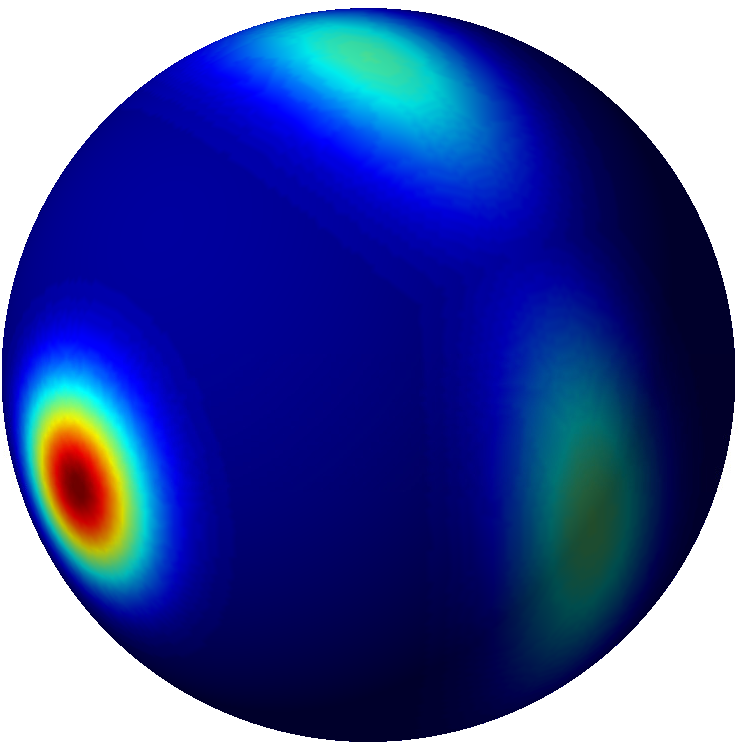
\includegraphics[width=1\columnwidth,height=0.4\textheight,keepaspectratio]{figures/2017AAS_matrix_fisher/TAC16_vis_3}};
% \draw[arrows={-Triangle[angle=30:4pt]}] (-2.1,-1.8) -- (-2.1,-1.2);
% \draw[arrows={-Triangle[angle=30:4pt]}] (-2.1,-1.8) -- (-2.5,-2.0);
% \draw[arrows={-Triangle[angle=30:4pt]}] (-2.1,-1.8) -- (-1.7,-2.0);
% \node at (-2.4,-2.15) {\scriptsize $e_1$};
% \node at (-1.7,-2.15) {\scriptsize $e_2$};
% \node at (-1.9,-1.4) {\scriptsize $e_3$};
\end{tikzpicture}
}
\centerline{\footnotesize $F_3=\mathrm{diag}[25,5,1]$}
\centerline{\footnotesize $U_3V_3^T=I_{3\times 3},\, U_3=I_{3\times 3}$}
\centerline{\footnotesize $S_3=\mathrm{diag}[25,5,1]$}
\end{column}
\end{columns}
\end{frame}

\begin{frame}
\frametitle{Attitude Estimation}

\begin{itemize}
\item \Emph{Attitude Estimation} Problem Formulation
	\begin{itemize}
	\item Consider a \Emph{stochastic differential equation}
	\[ (R^T dR)^\vee = \Omega dt + H dW,\]
	with a measured angular velocity $\Omega\in\Re^3$, a scaled Wiener process $HdW$ representing measurement noise
	\item Initial attitude follows a \Emph{matrix Fisher distribution}: $R(0)\sim\mathcal{M}(F(0))$
	\item Attitude is measured repeatedly
	\item \Emph{Goal}: determine the current distribution of the attitude uncertainty
	\end{itemize}
\vspace*{0.3cm}\pause
\item \Emph{Bayesian Estimation} with Matrix Fisher Distribution on $\SO$
	\begin{itemize}
	\item \Emph{Assumed density filter}: estimation constructed by $R(t)\sim\mathcal{M}(F(t))$
	\item \Emph{Propagation}
		\begin{itemize}
		\item First-order Propagation
		\item Unscented Transform
		\end{itemize}
	\item \Emph{Measurement Update}
	\end{itemize}
\end{itemize}
\end{frame}

\begin{frame}
\frametitle{Attitude Estimation}

\begin{itemize}
\item \Emph{First-Order Propagation}
	\begin{itemize}
	\item Suppose $R_k\sim\mathcal{M}(F_k)$ and $\Omega(t)$ is fixed over $[t_k,t_{k+1}]$
	\item From the Magnus expansion on $\SO$, the \Emph{first moment of $R_{k+1}$} is
	
\centerline{
    \begin{beamercolorbox}[wd=\textwidth,sep=0.0cm,center,rounded=true,shadow=true]{numerical}
	$\displaystyle
\mathrm{E}[R_{k+1}]= \mathrm{E}[R_k]\braces{I_{3\times 3}+\frac{h}{2}(-\trs{G_k}I_{3\times 3} + G_k)}\exp(h\hat\Omega_k) +\mathcal{O}(h^{1.5}),$	
\end{beamercolorbox}}
	where $G_k=hH_kH_k^T$
	\end{itemize}
\vspace*{0cm}\pause

\item Construct $\mathcal{M}(F_{k+1})$ to match $\mathrm{E}[R_{k+1}]$
	\begin{itemize}
	\item Perform the proper singular value decomposition to obtain 
	
\centerline{
    \begin{beamercolorbox}[wd=\textwidth,sep=0.0cm,center,rounded=true,shadow=true]{numerical}	
	$\mathrm{E}[R_{k+1}]=U_{k+1}\,\mathrm{diag}[d_1,d_2,d_3]\,V_{k+1}^T$
\end{beamercolorbox}}

	\item Recall the first moment of $R_{k+1}$ is given by
	
\centerline{
    \begin{beamercolorbox}[wd=\textwidth,sep=0.0cm,center,rounded=true,shadow=true]{numerical}
	$
\mathrm{E}[R_{k+1}]= U_{k+1}\, \mathrm{diag} \left[\frac{1}{c(S_{k+1})}\deriv{c(S_{k+1})}{s_1},\,
\frac{1}{c(S_{k+1})}\deriv{c(S_{k+1})}{s_2},\,\frac{1}{c(S_{k+1})}\deriv{c(S_{k+1})}{s_3}\right] \, V_{k+1}^T$	\end{beamercolorbox}}

	\item Solve $\frac{1}{c(S_{k+1})}\deriv{c(S_{k+1})}{s_1}=d_i$ for $S_{k+1}$
	\item Compute $F_{k+1}=U_{k+1} S_{k+1} V_{k+1}^T$ -- \Emph{Propagation to match the first moment}
	\item 
	\end{itemize}
\end{itemize}


\end{frame}
\begin{frame}
\frametitle{Measurement Update}

\begin{itemize}
\item Measurements
	\begin{itemize}
	\item \Emph{Full attitude measurement} $Z_i\in\SO$ for $i\in\{1,\ldots, N_Z\}$

\centerline{
    \begin{beamercolorbox}[wd=10cm,sep=0.0cm,center,rounded=true,shadow=true]{numerical}
	$\displaystyle
	Z_i|R \sim \mathcal{M}(F_{Z_i}),$
\end{beamercolorbox}}	

	where the matrix parameter $F_{Z_i}$ defines sensor uncertainty
\pause
\vspace*{0cm}
	\item \Emph{Direction measurement} $z_i\in\mathsf{S}^2$ for $i\in\{1,\ldots, N_z\}$ to a known reference direction $a_i$ follows the \Emph{von-Mises Fisher distribution on the unit-sphere},

\centerline{
    \begin{beamercolorbox}[wd=10cm,sep=0.0cm,center,rounded=true,shadow=true]{numerical}
	$\displaystyle
	p(z_i| R) =\frac{b_i}{4\pi \sinh b_i}\exp(b_i a_i^TB_i^T Rz_i),$
	\end{beamercolorbox}}	
	where $b_i\in\Re$ and $B_i\in\SO$ define sensor uncertainty
		
	\end{itemize}
\vspace*{0cm}\pause
\item Measurement Update
	\begin{itemize}
	\item The \Emph{a posteriori distribution} is also a matrix Fisher distribution
	
\centerline{
    \begin{beamercolorbox}[wd=10cm,sep=0.0cm,center,rounded=true,shadow=true]{numerical}
	$\displaystyle
R|(Z_1,\ldots, Z_{N_Z},z_1,\ldots z_{N_Z}) \sim \mathcal{M}(F + \sum_{i=1}^{N_Z} Z_iF_{Z_i}^T +\sum_{j=1}^{N_z} b_j B_j a_j z_j^T)$
	\end{beamercolorbox}}	
	
	\end{itemize}

\end{itemize}

\end{frame}

\begin{frame}
    \frametitle{Matrix Fisher mixture estimation}

    \begin{itemize}
        \item Mixture propagation  
        \begin{itemize}
            \item Prediction: $R_k\sim\mathcal{M}(\mathbf{F}_k,\boldsymbol{\alpha}_k)$ to $ R_{k+1} \sim \mathcal{M}(\mathbf{F}_{k+1},\boldsymbol{\alpha}_{k+1})$
            \item Assume weighting parameters constant over prediction: $\boldsymbol{\alpha}_{k+1}=\boldsymbol{\alpha}_{k}$
        \end{itemize}
        \centerline{
        \begin{beamercolorbox}[wd=10cm,sep=0.0cm,center,rounded=true,shadow=true]{numerical}
        \(\mathrm{E}[R_{k+1}] = \sum_{i=1}^n \alpha_{i_k}\, U_{i_{k+1}} \bar Q_{i_{k+1}} V_{i_{k+1}}^T +\mathcal{O}(h^{1.5}) \)
        \end{beamercolorbox}}
        \pause
        \item Measurement uncertainty
        \begin{itemize}
            \item Full attitude sensor measurement \( Z \in \SO \)
            \item Measurement error \( R^T Z \in \SO \sim \mathcal{M}(\mathbf{G},\boldsymbol{\beta})\)
        \end{itemize}
        \centerline{
        \begin{beamercolorbox}[wd=10cm,sep=0.0cm,center,rounded=true,shadow=true]{numerical}
        \( p(Z|R) = \sum_{j=1}^m\frac{\beta_j}{c(G_j)} \exp(\trs{G_j^T R^T Z}) \)
        \end{beamercolorbox}}
        \pause
        \item Measurement Update
        \begin{itemize}
            \item The \Emph{a posteriori distribution} is also a matrix Fisher mixture
        \end{itemize}
        \centerline{
        \begin{beamercolorbox}[wd=10cm,sep=0.0cm,center,rounded=true,shadow=true]{numerical}
        \( R|Z\sim\mathcal{M}(\mathbf{H}, \boldsymbol{\gamma}), \)
        \end{beamercolorbox}}
    \end{itemize}
\end{frame}

\begin{frame}
\frametitle{Numerical Example}

\begin{itemize}
\item True Attitude Trajectory
    \begin{center}
    \animategraphics[controls,autoplay,loop,width=0.5\textwidth, height=0.5\textheight,keepaspectratio]{8}{animation/3Dpend/3Dpend_}{1}{1958}
\end{center}
\pause
\item Measurement
	\begin{itemize}
	\item Angular velocity: $50\,\mathrm{Hz}$ with the mean error of $0.45\,\mathrm{rad/s}$
	\item Attitude: $10\,\mathrm{Hz}$ with the mean errr of $10.04^\circ$
	\end{itemize}
\end{itemize}


\end{frame}


\begin{frame}
\frametitle{Numerical Example}

\only<1>{
\begin{itemize}
\item Single matrix Fisher: \quad \Emph{large initial error} with $F(0)=100\exp (\pi\hat e_1)$
	\begin{itemize}
	\item Initial error: $180^\circ$, Initial singular values $s=100$
	\item \Emph{Falsely too confident} about the \Emph{completely wrong attitude}
	\end{itemize}
\end{itemize}


\begin{figure}\setcounter{subfigure}{0}
\centerline{
    \subcaptionbox{ Attitude estimation error ($\mathrm{deg}$) }[0.5\textwidth]{\hspace*{0.03\columnwidth}
		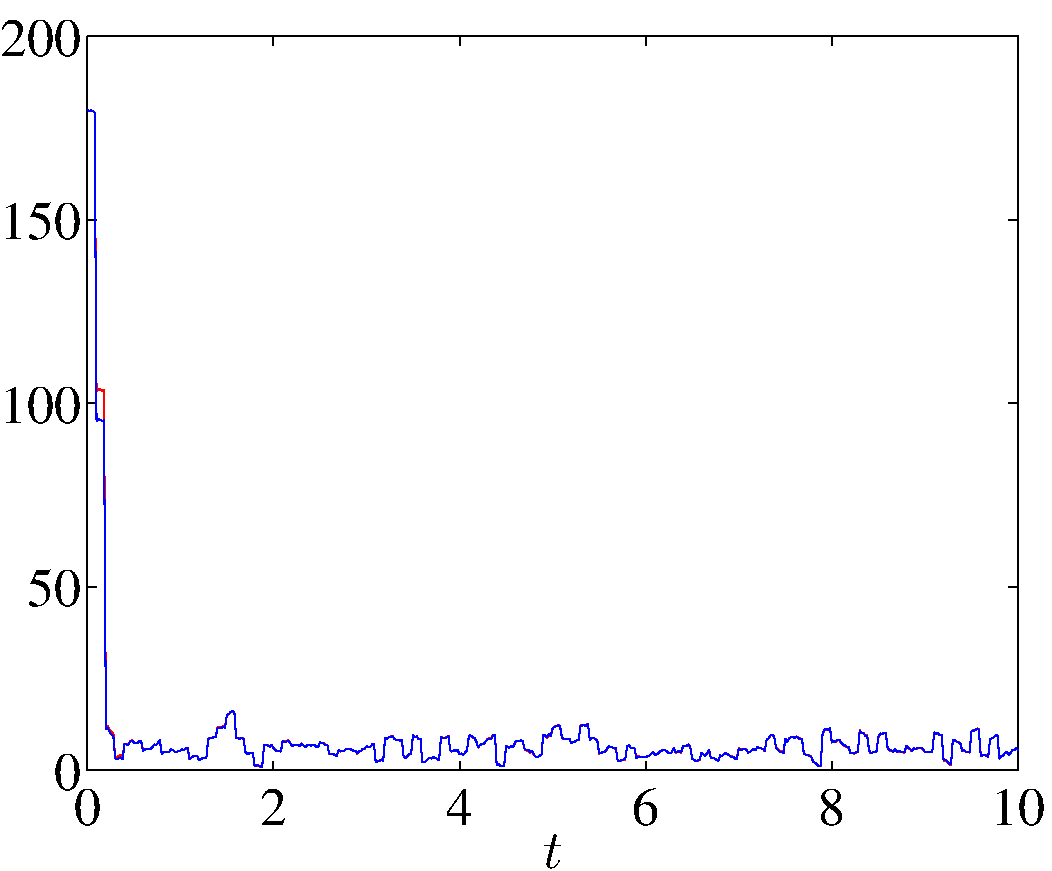
\includegraphics[height=0.6\textheight,width=0.5\textwidth,keepaspectratio]{figures/2017AAS_matrix_fisher/TAC16_0_R_est_err}\label{fig:R_est_err_0}\hspace*{0.03\columnwidth}}~
                \subcaptionbox{ Uncertainty measured by $\frac{1}{s_i+s_j}$ }[0.5\textwidth]{
		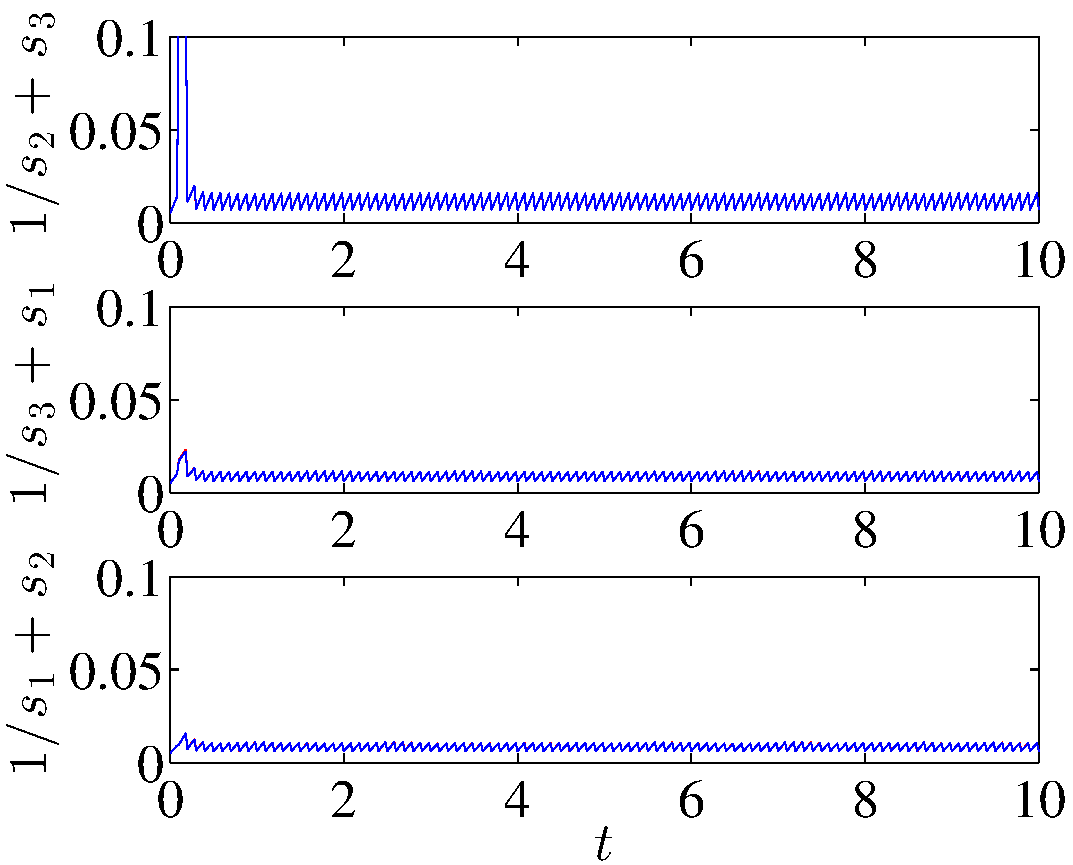
\includegraphics[height=0.6\textheight,width=0.5\textwidth,keepaspectratio]{figures/2017AAS_matrix_fisher/TAC16_0_s}}
}
\end{figure}}

\only<2>{
    \tiny
\begin{figure}
    \centering
    \subcaptionbox{ \tiny $t=0$,~$p_{\max}=1.45\times 10^4$ }[0.33\textwidth]{
        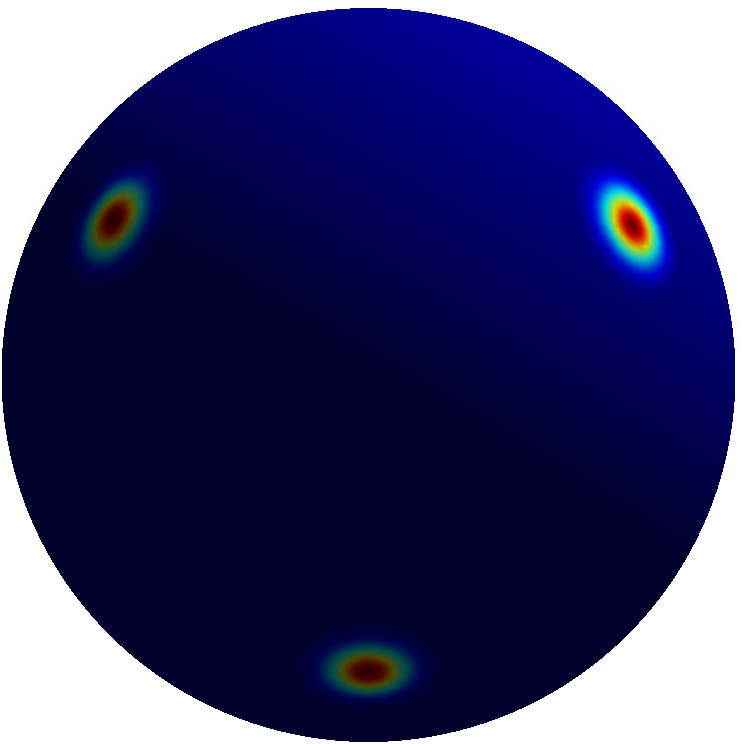
\includegraphics[width=0.4\textwidth,height=0.35\textheight,keepaspectratio]{figures/2017AAS_matrix_fisher/TAC16_0_F_1b}}~
    \subcaptionbox{ \tiny $t=0.08$, $p_{\max}=4.38\times 10^3$ }[0.33\textwidth]{
        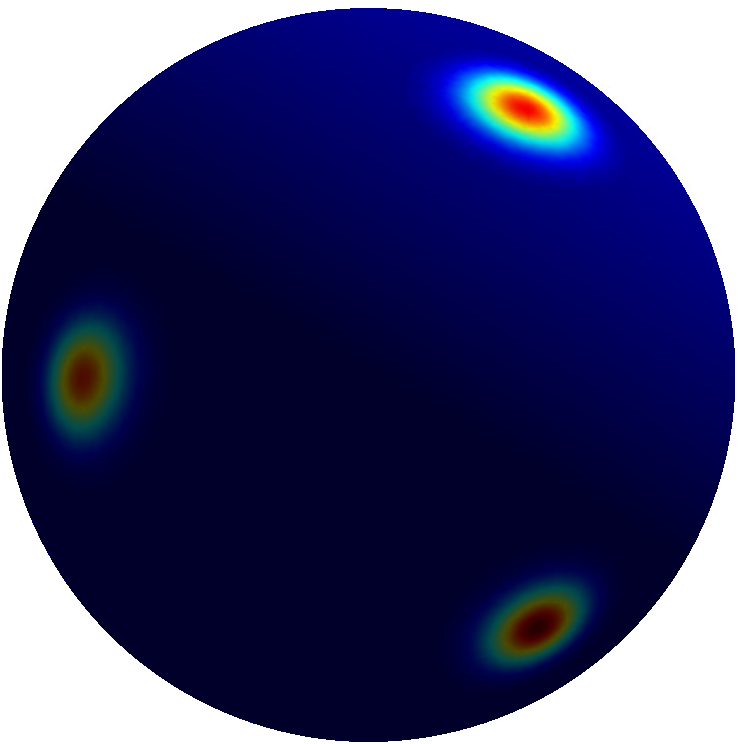
\includegraphics[width=0.33\textwidth,height=0.35\textheight,keepaspectratio]{figures/2017AAS_matrix_fisher/TAC16_0_F_5b}}~
    \subcaptionbox{ \tiny $t=0.1$, $p_{\max}=1.08\times 10^{3}$ }[0.33\textwidth]{
            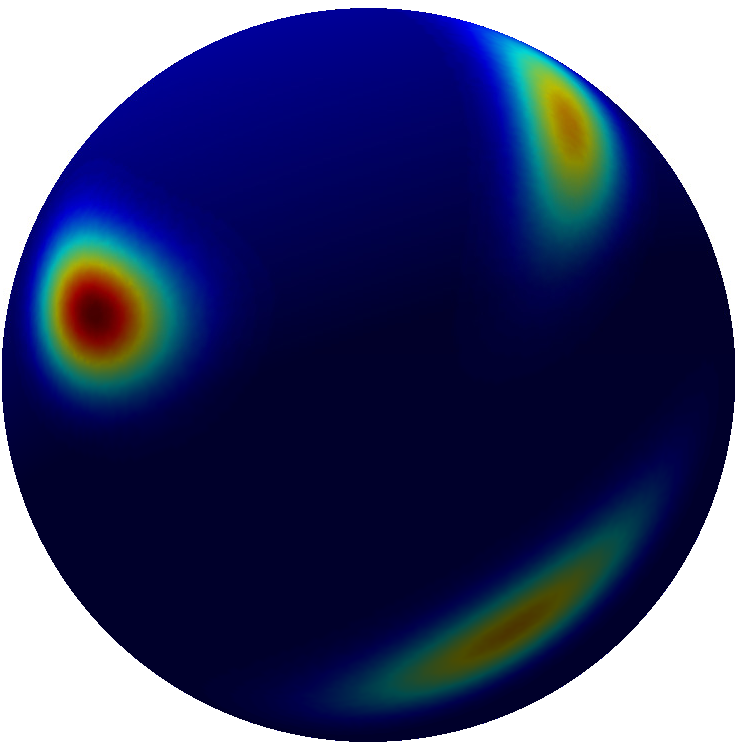
\includegraphics[width=0.33\textwidth, height=0.35\textheight, keepaspectratio]{figures/2017AAS_matrix_fisher/TAC16_0_F_6b}}\\
    \subcaptionbox{ \tiny $t=0.3$, $p_{\max}=8.73\times 10^3$ }[0.33\textwidth]{
        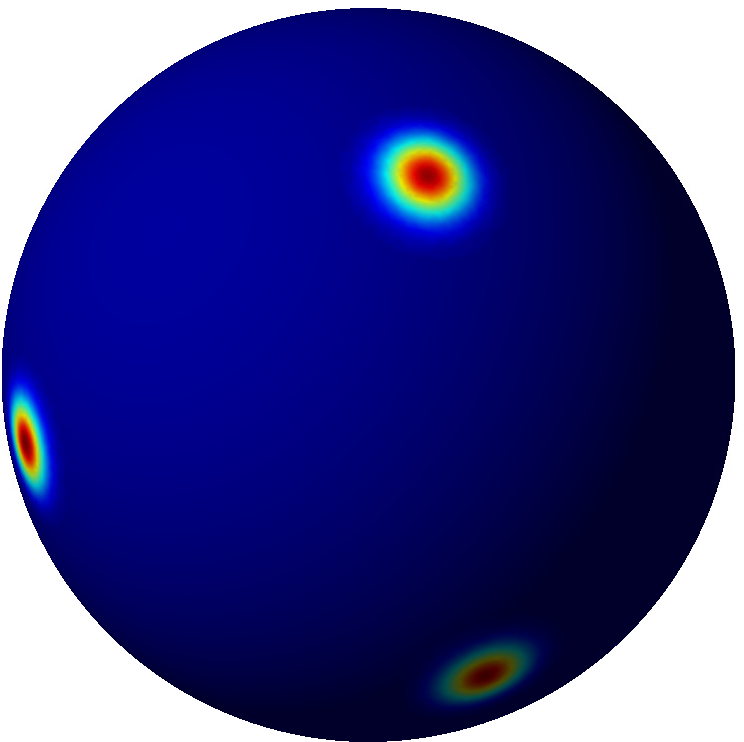
\includegraphics[width=0.33\textwidth,height=0.35\textheight,keepaspectratio]{figures/2017AAS_matrix_fisher/TAC16_0_F_16b}}~
    \subcaptionbox{\tiny $t=1$, $p_{\max}=9.61\times 10^3$ }[0.33\textwidth]{
        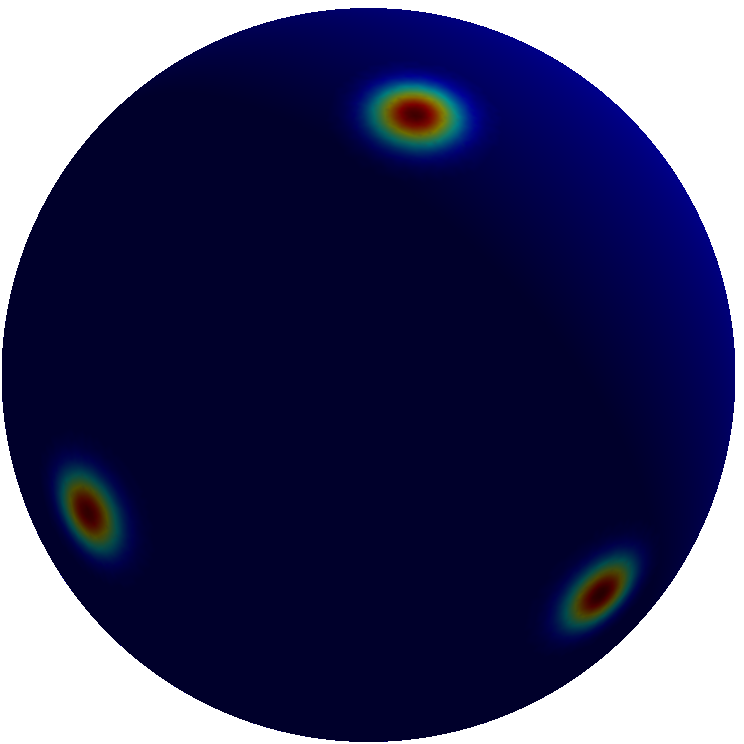
\includegraphics[width=0.33\textwidth,height=0.35\textheight,keepaspectratio]{figures/2017AAS_matrix_fisher/TAC16_0_F_51b}}~
    \subcaptionbox{\tiny $t=10$, $p_{\max}=9.82\times 10^3$ }[0.33\textwidth]{
        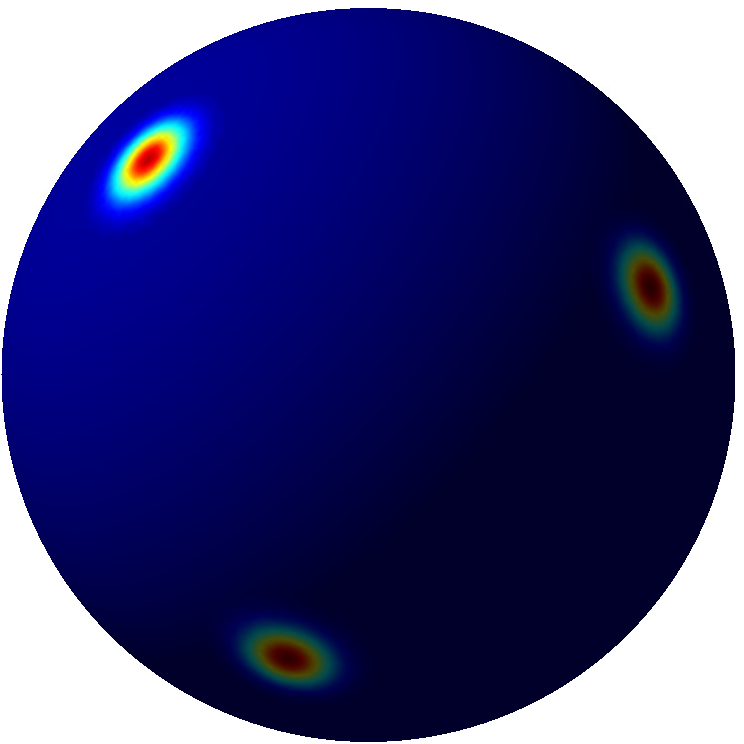
\includegraphics[width=0.33\textwidth,height=0.35\textheight,keepaspectratio]{figures/2017AAS_matrix_fisher/TAC16_0_F_501b}}
    \caption{Case I: visualizations of $\mathcal{M}(F_k)$ for the first-order filter}\label{fig:visES_0}
\end{figure}
}

\end{frame}

\begin{frame}
\frametitle{Numerical Example}

\only<1>{
\begin{itemize}
\item Matrix Fisher mixture: \Emph{large uncertainty} with three components
	\begin{itemize}
        \item True initial attitude: $R_{true}(0)=I_{3\times 3}$ and estimator is biased by three inaccurate estimates with large errors
	    \item Initially uncertain of rotation about first body fixed axis
	\end{itemize}
\end{itemize}

\begin{columns}
\begin{column}{0.5\textwidth}
    {\small
    \begin{gather*}
F_{1_0} = 20 \exp (\frac{1}{3}\pi\hat e_1),\quad \alpha_{1_0}=\frac{1}{4}, \\
F_{2_0} = 20 \exp (\frac{2}{3}\pi\hat e_1),\quad \alpha_{2_0}=\frac{1}{2}, \\
F_{3_0} = 20 \exp (\pi\hat e_1)\quad \alpha_{3_0}=\frac{1}{4}.
\end{gather*}}
\end{column}
\begin{column}{0.5\textwidth}
\begin{figure}\setcounter{subfigure}{0}
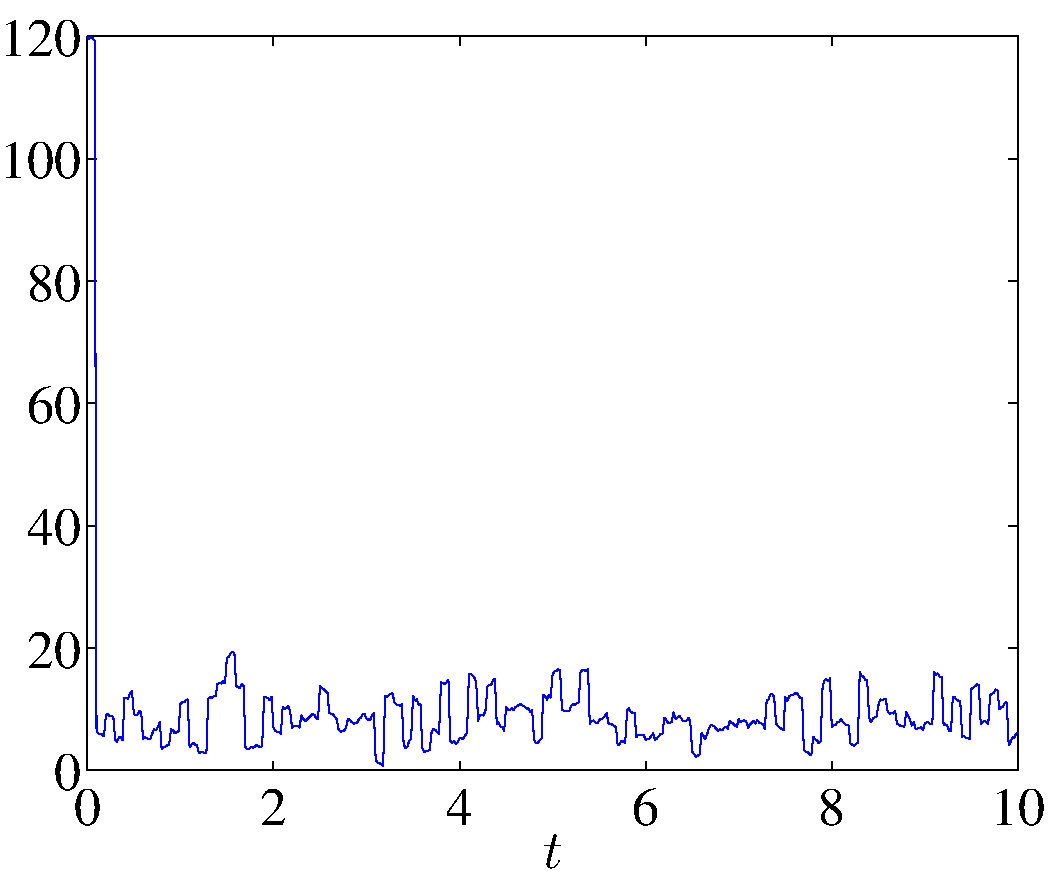
\includegraphics[width=\textwidth,height=0.65\textheight,keepaspectratio]{figures/2017AAS_matrix_fisher/AAS17_1_R_est_err} 
\end{figure}
\end{column}
\end{columns}
}

\only<2>{
\begin{figure}
	\subcaptionbox{ \tiny $t=0$, $p_{mse}=6.47\times 10^-7$ }[0.33\textwidth]{
		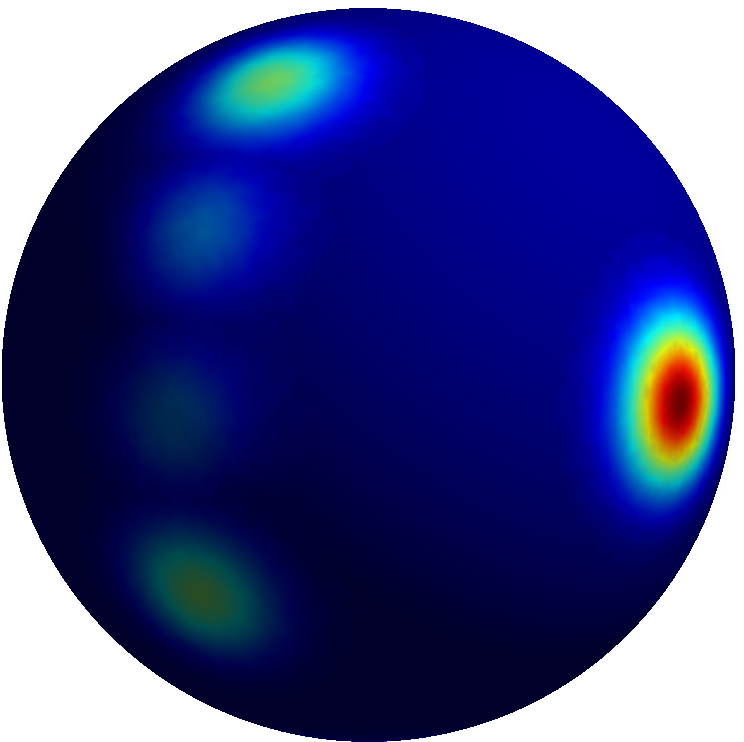
\includegraphics[width=0.33\textwidth,height=0.35\textheight,keepaspectratio]{figures/2017AAS_matrix_fisher/est_MF_mix_AAS17_1_1}}~
	\subcaptionbox{ \tiny $t=0.06$, $p_{mse}=3.4\times 10^-3$ }[0.33\textwidth]{
		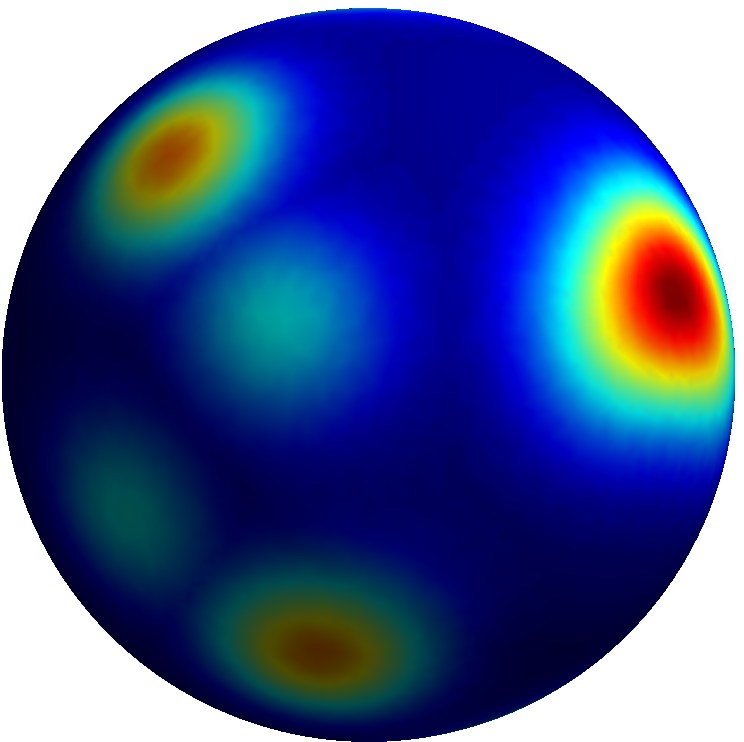
\includegraphics[width=0.33\textwidth,height=0.35\textheight,keepaspectratio]{figures/2017AAS_matrix_fisher/est_MF_mix_AAS17_1_4}}~
	\subcaptionbox{ \tiny $t=0.08$, $p_{mse}=4.2\times 10^{-3}$ }[0.33\textwidth]{
		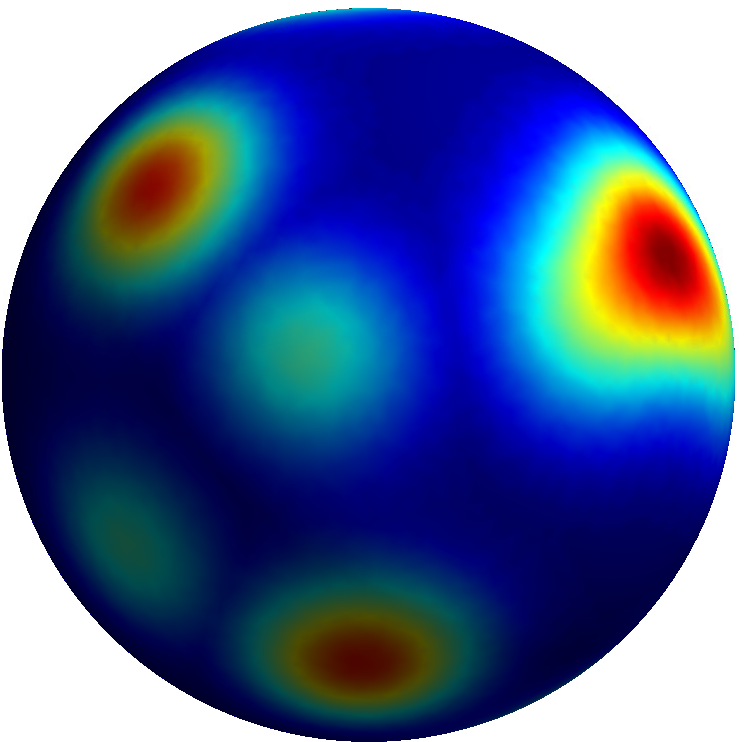
\includegraphics[width=0.33\textwidth,height=0.35\textheight,keepaspectratio]{figures/2017AAS_matrix_fisher/est_MF_mix_AAS17_1_5}}\\
	\subcaptionbox{ \tiny $t=0.1$, $p_{mse}=1.08\times 10^3$ }[0.33\textwidth]{
		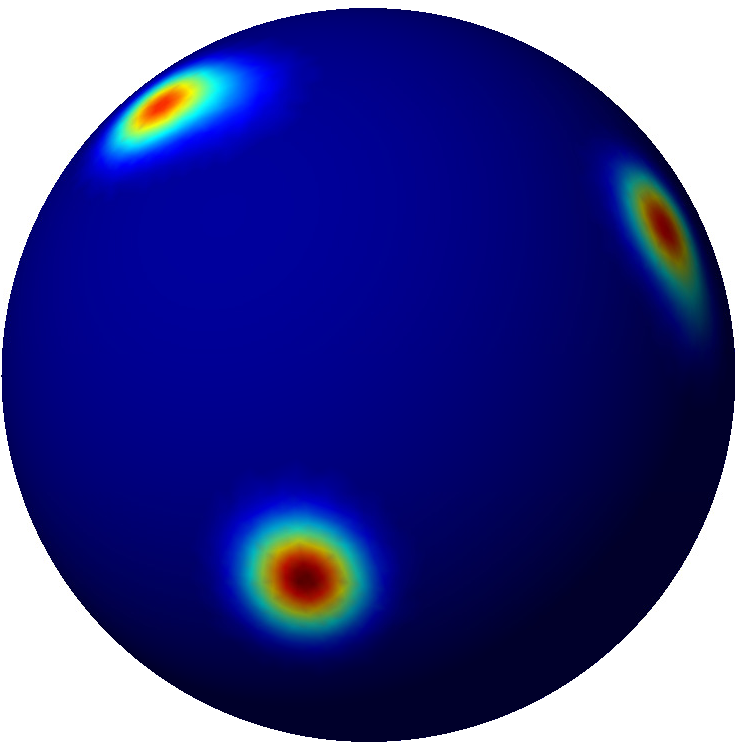
\includegraphics[width=0.33\textwidth,height=0.35\textheight,keepaspectratio]{figures/2017AAS_matrix_fisher/est_MF_mix_AAS17_1_6}}~
	\subcaptionbox{ \tiny $t=2$, $p_{mse}=1.29\times 10^3$ }[0.33\textwidth]{
		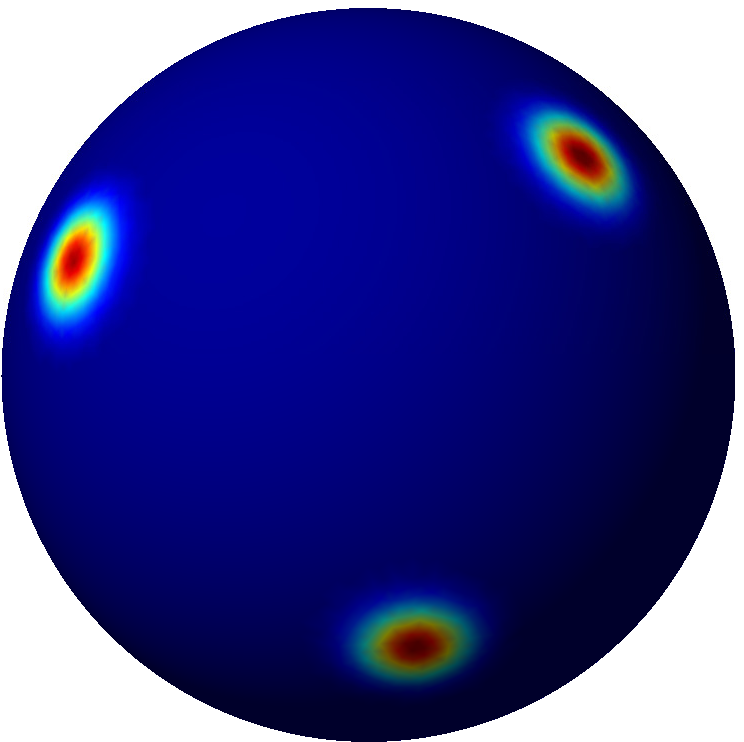
\includegraphics[width=0.33\textwidth,height=0.35\textheight,keepaspectratio]{figures/2017AAS_matrix_fisher/est_MF_mix_AAS17_1_11}}~
	\subcaptionbox{ \tiny $t=10$, $p_{mse}=1.29\times 10^3$ }[0.33\textwidth]{
		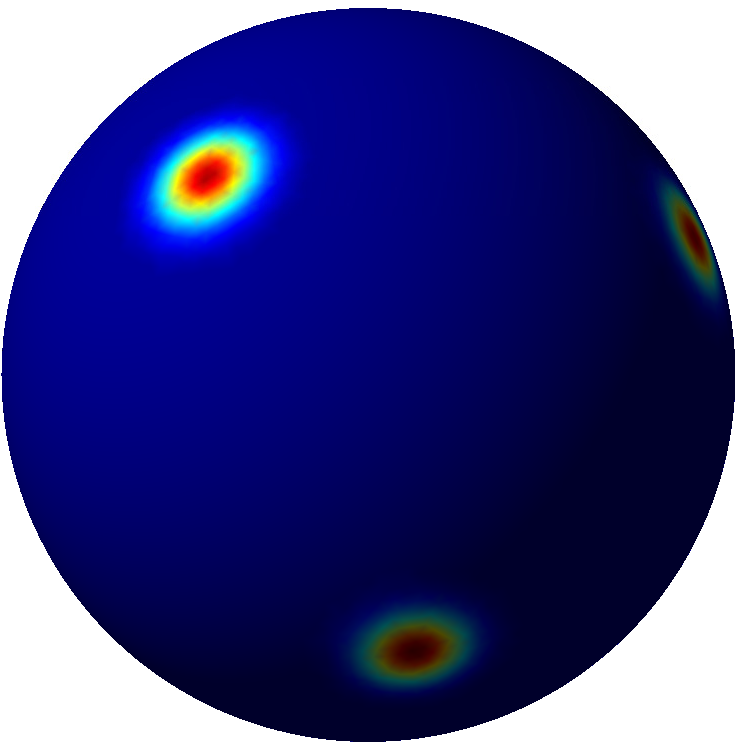
\includegraphics[width=0.33\textwidth,height=0.35\textheight,keepaspectratio]{figures/2017AAS_matrix_fisher/est_MF_mix_AAS17_1_501}}
\end{figure}
}

\end{frame}
